\documentclass[12pt,a4paper]{article}

% ============================================================
% Packages
% ============================================================
\usepackage[T1]{fontenc}
\usepackage[utf8]{inputenc}
\usepackage{geometry}
\usepackage{graphicx}
\usepackage{amsmath,amssymb}
\usepackage{xcolor}
\usepackage{physics}
\usepackage{listings}
\usepackage{hyperref}
\usepackage{float}
\setlength{\intextsep}{10pt plus 2pt minus 2pt}



\geometry{margin=1in}

% ============================================================
% Python code style
% ============================================================
\lstdefinestyle{pythonstyle}{
  language=Python,
  basicstyle=\ttfamily\small,
  keywordstyle=\color{blue}\bfseries,
  commentstyle=\color{teal!70!black}\itshape,
  stringstyle=\color{purple},
  showstringspaces=false,
  frame=single,
  numbers=left,
  numberstyle=\tiny,
  breaklines=true,
  tabsize=4,
  upquote=true
}

% ============================================================
% Document starts
% ============================================================
\begin{document}

\title{\textbf{Binary Population Simulation and Gravitational Wave Merger Modelling}}\\[6pt]
%\large Computational Project based on MSc Research at Queen Mary University of London}
\author{Devika Chandiran - MSc Astrophysics, Queen Mary University of London}
\date{October 2025}
\makeatletter
\renewenvironment{abstract}{%
    \small
    \begin{center}
      {\bfseries \abstractname\vspace{-.5em}\vspace{\z@}}
    \end{center}
    \list{}{\leftmargin=0.0cm \rightmargin=0.0cm}
    \item\relax
}{\endlist}
\makeatother

\maketitle

\begin{abstract}
    

    

This report describes a numerical simulation of compact binary systems and their evolution due to gravitational wave emission. The work extends my MSc research project at Queen Mary University of London. Using a simple model based on Peters (1964), the simulation estimates merger times, chirp masses and statistical properties of the population. All equations and results are explained in clear and direct terms for accessibility.
\end{abstract}

% ============================================================
\section{Introduction}
Gravitational waves provide a direct way to study compact binaries such as black holes and neutron stars. 
When two massive bodies orbit one another, they emit energy as gravitational radiation, which gradually reduces the orbital separation until they merge. 
The rate at which this happens depends mainly on the component masses and their initial distance. 
In this project I created a Python model that generates a random population of binaries and computes their merger times and chirp masses, showing which systems would merge within the lifetime of the Universe.

% ============================================================
\section{Physical Background}
For a circular binary with component masses $m_1$ and $m_2$, and an initial orbital separation $a_0$, the time until coalescence due to gravitational wave radiation is given by Peters (1964) as:
\begin{equation}
t_{\text{merge}} = \frac{5}{256}\frac{c^5 a_0^4}{G^3 m_1 m_2 (m_1 + m_2)}.
\end{equation}

This equation shows that tighter and more massive systems merge faster.  
The \textit{chirp mass}, which affects the observed gravitational wave frequency and amplitude, is defined as:
\begin{equation}
\mathcal{M} = \frac{(m_1 m_2)^{3/5}}{(m_1 + m_2)^{1/5}}.
\end{equation}

These two quantities are key to understanding gravitational wave signals and the detectability of sources.

% ============================================================
\section{Numerical Implementation}

\subsection{Setup and Constants}
\begin{lstlisting}[style=pythonstyle]
import numpy as np
import matplotlib.pyplot as plt
from scipy.constants import G, c
import os

# Physical constants
YEAR = 365.25 * 24 * 3600        # seconds in a year
MSUN = 1.98847e30                # kilograms in one solar mass
RSUN = 6.957e8                   # metres in one solar radius

plt.rcParams.update({'figure.figsize': (7, 5), 'axes.grid': True})
print("Environment ready")
\end{lstlisting}

\subsection{Sampling Binary Systems}
\begin{lstlisting}[style=pythonstyle]
def sample_m1(size, mmin=5, mmax=40, alpha=2.35):
    """
    Draws the primary mass using a Salpeter power law.
    """
    r = np.random.rand(size)
    a1 = 1 - alpha
    return ((r * (mmax**a1 - mmin**a1) + mmin**a1)) ** (1 / a1)

N = 5000  # number of binaries
m1 = sample_m1(N)
q = np.random.uniform(0.3, 1.0, N)  # mass ratio
m2 = q * m1
a0 = np.exp(np.random.uniform(np.log(1), np.log(100), N))  # separation in solar radii

print(f"Generated {N} binary systems")
\end{lstlisting}

\subsection{Merger Time and Chirp Mass}
\begin{lstlisting}[style=pythonstyle]
def merger_time_s(m1_msun, m2_msun, a0_rsun):
    """
    Calculates the merger time for circular binaries in seconds.
    """
    m1, m2, a0 = m1_msun * MSUN, m2_msun * MSUN, a0_rsun * RSUN
    num = 5 * c**5 * a0**4
    den = 256 * G**3 * m1 * m2 * (m1 + m2)
    return num / den

tmerge_s = merger_time_s(m1, m2, a0)
tmerge_yr = tmerge_s / YEAR

def chirp_mass(m1, m2):
    M = m1 + m2
    return (m1 * m2)**(3/5) / (M**(1/5))

chirp = chirp_mass(m1, m2)

HUBBLE_TIME_YR = 13.8e9
merge_mask = tmerge_yr < HUBBLE_TIME_YR
print(f"{merge_mask.sum()} binaries merge within a Hubble time")
\end{lstlisting}

\subsection{Visualisation of Results}
\begin{lstlisting}[style=pythonstyle]
os.makedirs("results", exist_ok=True)

# Plot 1: Merger time distribution
plt.figure()
plt.hist(np.log10(tmerge_yr[merge_mask]), bins=40,
         colour="steelblue", edgecolour="black")
plt.xlabel("log10 Merger Time [years]")
plt.ylabel("Number of systems")
plt.title("Merger Time Distribution (within 13.8 Gyr)")
plt.tight_layout()
plt.savefig("results/merger_times_hist.png", dpi=160)
plt.show()

# Plot 2: Chirp mass versus merger time
plt.figure()
plt.scatter(tmerge_yr[merge_mask], chirp[merge_mask],
            s=6, alpha=0.7, colour="darkorange")
plt.xscale("log")
plt.xlabel("Merger Time [years] (log scale)")
plt.ylabel("Chirp Mass [Solar Masses]")
plt.title("Chirp Mass vs Merger Time")
plt.tight_layout()
plt.savefig("results/chirp_vs_tmerge.png", dpi=160)
plt.show()

# Plot 3: Component masses
plt.figure()
plt.scatter(m1, m2, s=4, alpha=0.4, colour="seagreen")
plt.xlabel("m1 [Solar Masses]")
plt.ylabel("m2 [Solar Masses]")
plt.title("Component Masses of All Systems")
plt.tight_layout()
plt.savefig("results/mass_scatter.png", dpi=160)
plt.show()

print("Simulation complete")
\end{lstlisting}

% ============================================================
\section{Results and Discussion}
Figure~\ref{fig1} shows the distribution of merger times for all systems that merge within the age of the Universe. 
Most binaries have very long inspiral times, while a smaller fraction merge in less than a billion years.  
Figure~\ref{fig2} plots chirp mass against merger time and shows that heavier systems merge more quickly.  
Figure~\ref{fig3} shows the range of component masses for all simulated binaries.

These patterns are consistent with physical expectations and with more detailed population synthesis results in the literature.  
This simple model therefore captures the essential physical relationships in a clear way.

\begin{figure}[H]

\centering
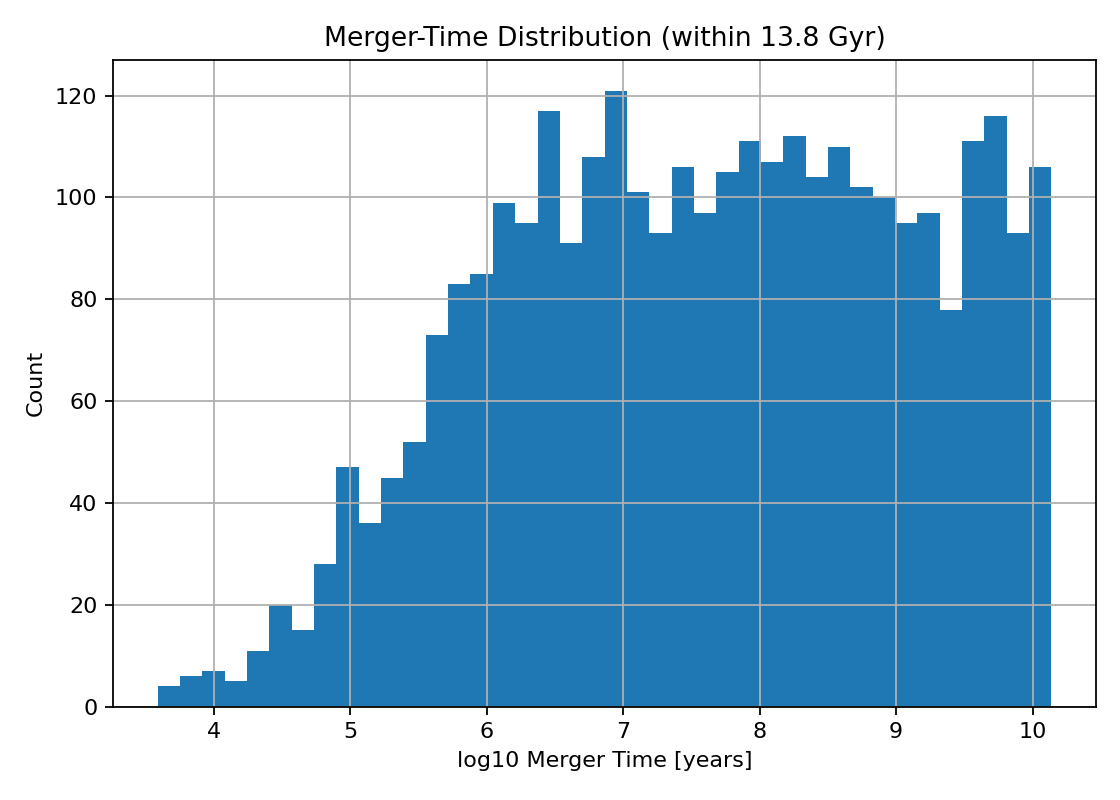
\includegraphics[width=0.65\textwidth]{merger_times_hist.png}
\caption{Distribution of merger times (log scale).}
\label{fig1}
\end{figure}

\begin{figure}[H]

\centering
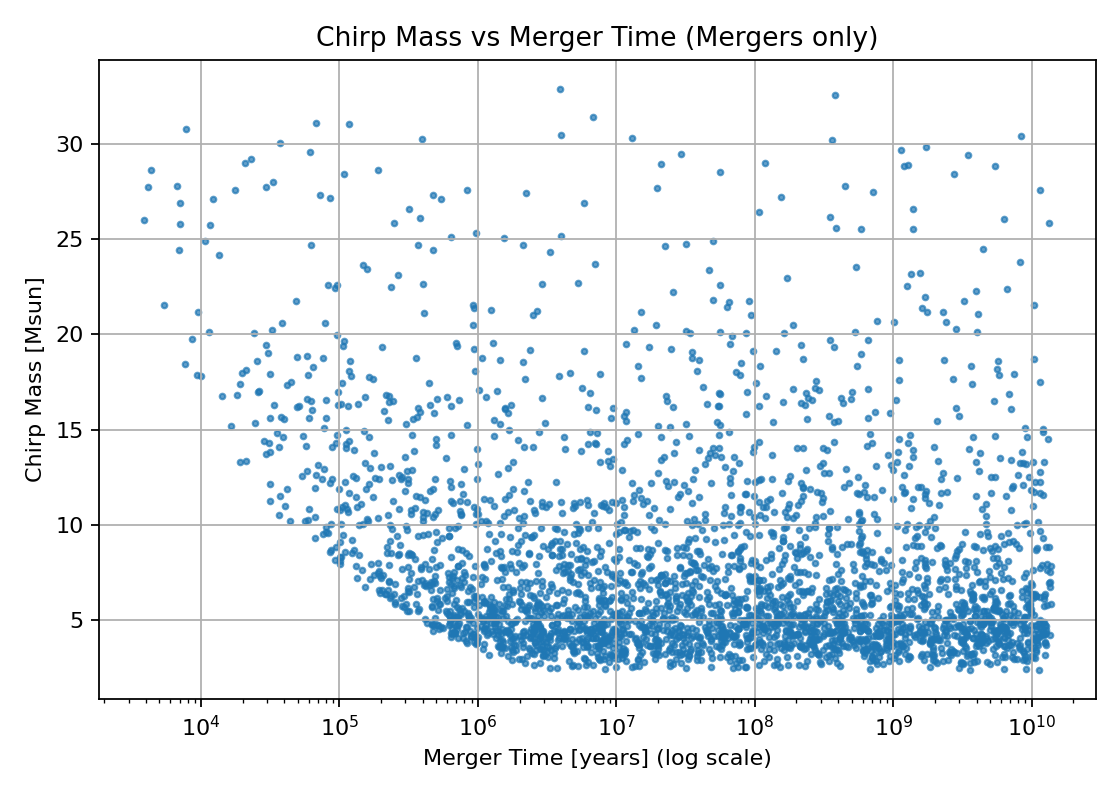
\includegraphics[width=0.65\textwidth]{chirp_vs_tmerge.png}
\caption{Chirp mass as a function of merger time.}
\label{fig2}
\end{figure}

\begin{figure}[H]

\centering
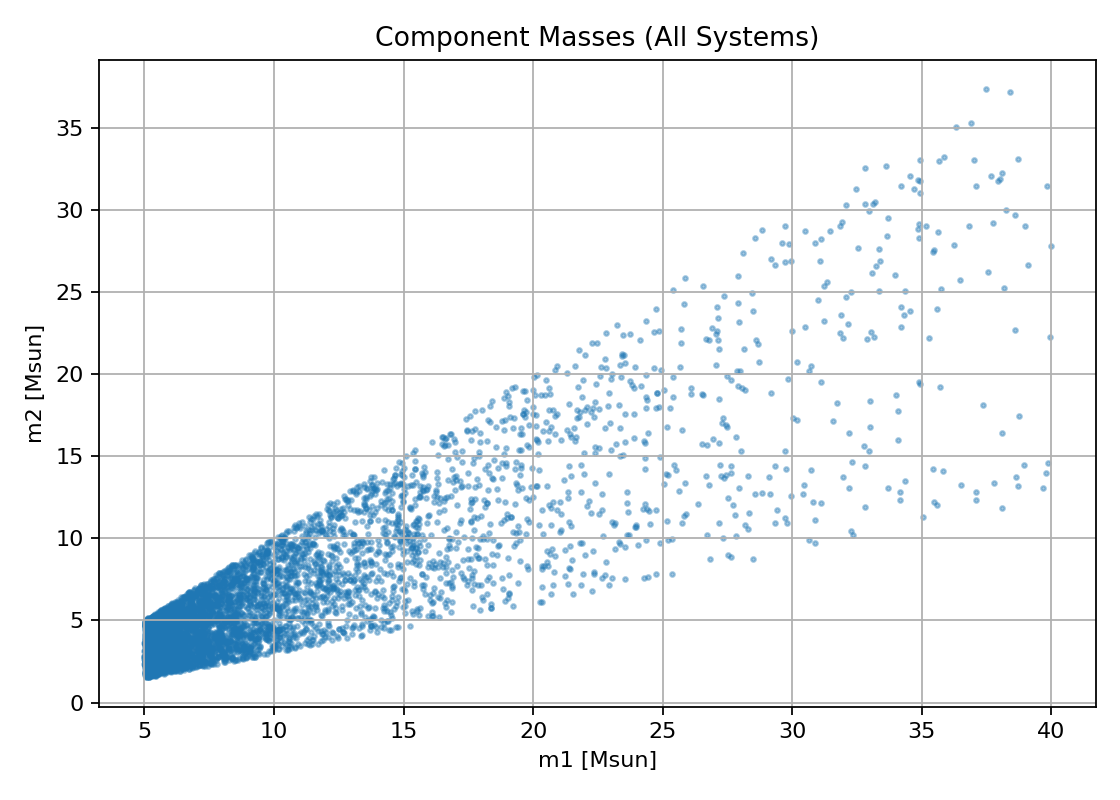
\includegraphics[width=0.65\textwidth]{mass_scatter.png}
\caption{Component masses of all systems.}
\label{fig3}
\end{figure}

% ============================================================
\section{Conclusion}
This project extends my MSc research and demonstrates how gravitational wave radiation influences the evolution of binary systems. 
Although the model is simple, it reproduces the main physical trends and builds a foundation for further work. 
In future, this can be developed to include metallicity, stellar winds and eccentricity, which would connect closely with the population synthesis research carried out at Radboud University. 
I am particularly interested in expanding this work to explore how binary evolution models can inform gravitational wave detections and source formation studies within the IMAPP group.


% ============================================================
\section*{Acknowledgement}
This work builds upon my MSc research at Queen Mary University of London.  
It reflects my continuing interest in computational astrophysics and gravitational wave cosmology.

% ============================================================
\section*{References}
\noindent Peters, P.C. (1964). \textit{Gravitational Radiation and the Motion of Two Point Masses}. Physical Review, 136(4B), B1224.\\
Cutler, C. and Thorne, K.S. (2002). \textit{An Overview of Gravitational Wave Sources}. arXiv:gr-qc/0204090.\\
Maggiore, M. (2008). \textit{Gravitational Waves: Volume 1}. Oxford University Press.

\end{document}
